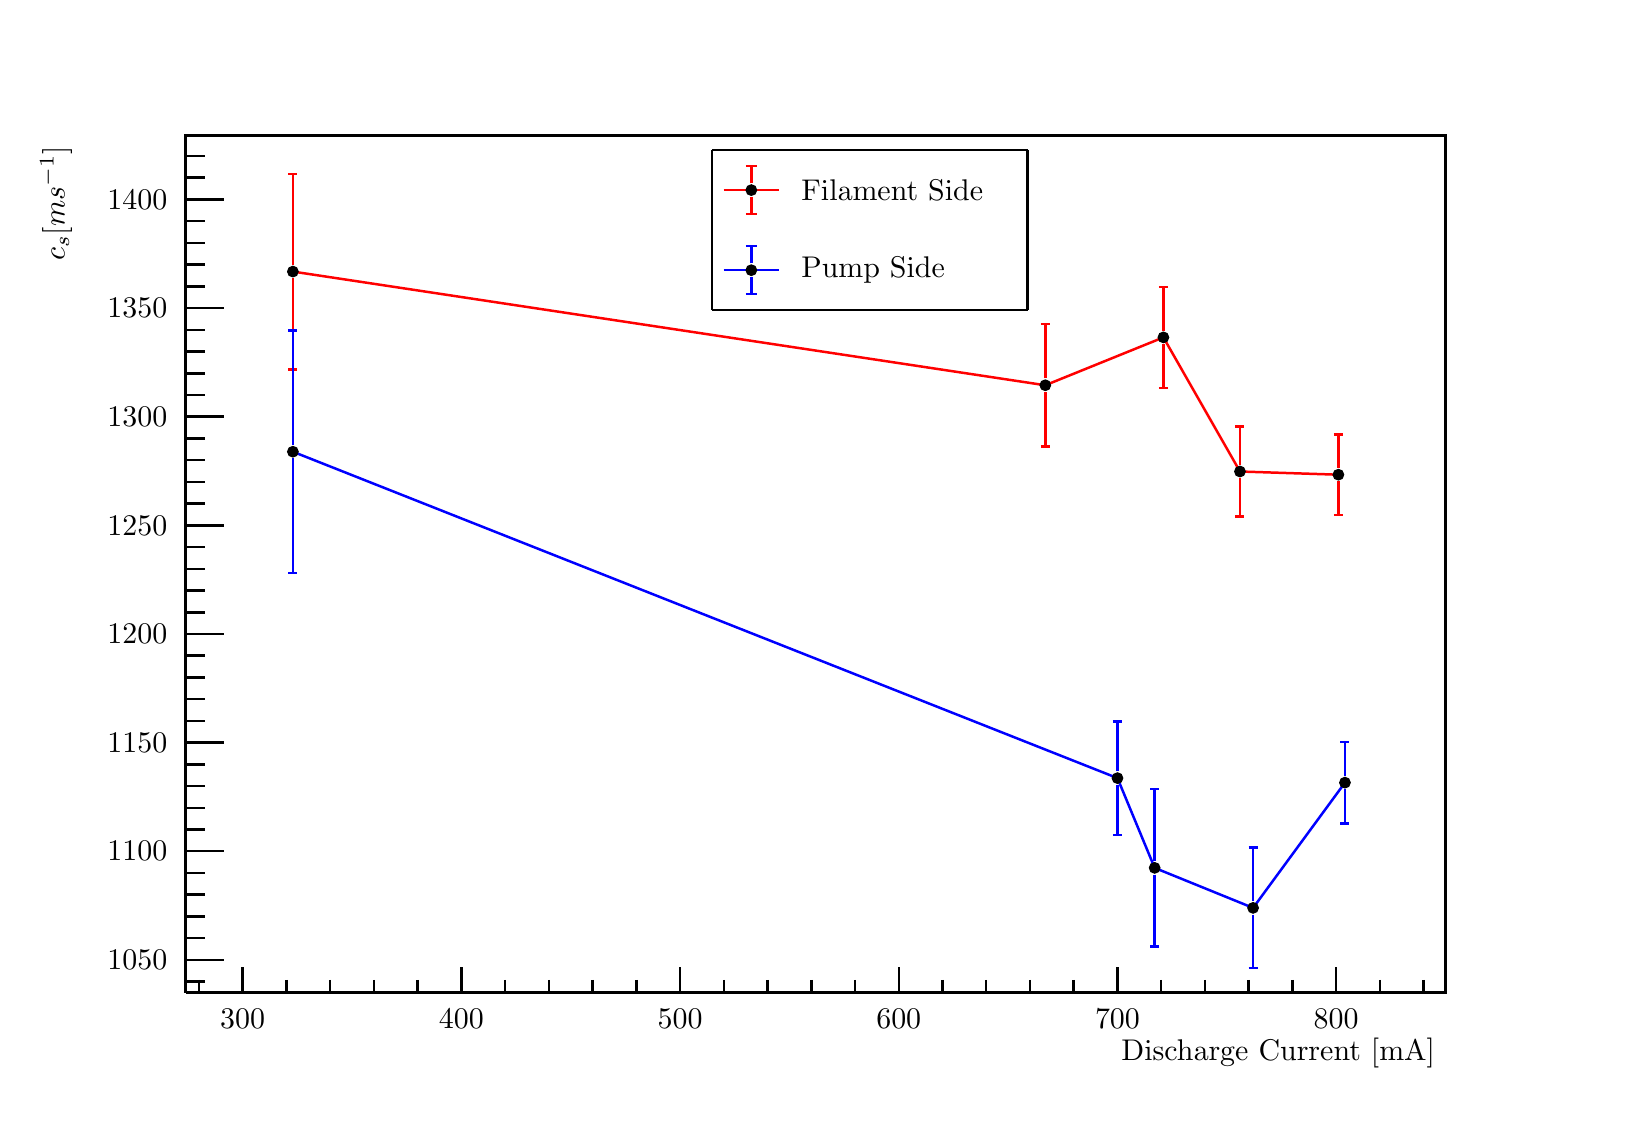
\begin{tikzpicture}
\pgfdeclareplotmark{cross} {
\pgfpathmoveto{\pgfpoint{-0.3\pgfplotmarksize}{\pgfplotmarksize}}
\pgfpathlineto{\pgfpoint{+0.3\pgfplotmarksize}{\pgfplotmarksize}}
\pgfpathlineto{\pgfpoint{+0.3\pgfplotmarksize}{0.3\pgfplotmarksize}}
\pgfpathlineto{\pgfpoint{+1\pgfplotmarksize}{0.3\pgfplotmarksize}}
\pgfpathlineto{\pgfpoint{+1\pgfplotmarksize}{-0.3\pgfplotmarksize}}
\pgfpathlineto{\pgfpoint{+0.3\pgfplotmarksize}{-0.3\pgfplotmarksize}}
\pgfpathlineto{\pgfpoint{+0.3\pgfplotmarksize}{-1.\pgfplotmarksize}}
\pgfpathlineto{\pgfpoint{-0.3\pgfplotmarksize}{-1.\pgfplotmarksize}}
\pgfpathlineto{\pgfpoint{-0.3\pgfplotmarksize}{-0.3\pgfplotmarksize}}
\pgfpathlineto{\pgfpoint{-1.\pgfplotmarksize}{-0.3\pgfplotmarksize}}
\pgfpathlineto{\pgfpoint{-1.\pgfplotmarksize}{0.3\pgfplotmarksize}}
\pgfpathlineto{\pgfpoint{-0.3\pgfplotmarksize}{0.3\pgfplotmarksize}}
\pgfpathclose
\pgfusepathqstroke
}
\pgfdeclareplotmark{cross*} {
\pgfpathmoveto{\pgfpoint{-0.3\pgfplotmarksize}{\pgfplotmarksize}}
\pgfpathlineto{\pgfpoint{+0.3\pgfplotmarksize}{\pgfplotmarksize}}
\pgfpathlineto{\pgfpoint{+0.3\pgfplotmarksize}{0.3\pgfplotmarksize}}
\pgfpathlineto{\pgfpoint{+1\pgfplotmarksize}{0.3\pgfplotmarksize}}
\pgfpathlineto{\pgfpoint{+1\pgfplotmarksize}{-0.3\pgfplotmarksize}}
\pgfpathlineto{\pgfpoint{+0.3\pgfplotmarksize}{-0.3\pgfplotmarksize}}
\pgfpathlineto{\pgfpoint{+0.3\pgfplotmarksize}{-1.\pgfplotmarksize}}
\pgfpathlineto{\pgfpoint{-0.3\pgfplotmarksize}{-1.\pgfplotmarksize}}
\pgfpathlineto{\pgfpoint{-0.3\pgfplotmarksize}{-0.3\pgfplotmarksize}}
\pgfpathlineto{\pgfpoint{-1.\pgfplotmarksize}{-0.3\pgfplotmarksize}}
\pgfpathlineto{\pgfpoint{-1.\pgfplotmarksize}{0.3\pgfplotmarksize}}
\pgfpathlineto{\pgfpoint{-0.3\pgfplotmarksize}{0.3\pgfplotmarksize}}
\pgfpathclose
\pgfusepathqfillstroke
}
\pgfdeclareplotmark{newstar} {
\pgfpathmoveto{\pgfqpoint{0pt}{\pgfplotmarksize}}
\pgfpathlineto{\pgfqpointpolar{44}{0.5\pgfplotmarksize}}
\pgfpathlineto{\pgfqpointpolar{18}{\pgfplotmarksize}}
\pgfpathlineto{\pgfqpointpolar{-20}{0.5\pgfplotmarksize}}
\pgfpathlineto{\pgfqpointpolar{-54}{\pgfplotmarksize}}
\pgfpathlineto{\pgfqpointpolar{-90}{0.5\pgfplotmarksize}}
\pgfpathlineto{\pgfqpointpolar{234}{\pgfplotmarksize}}
\pgfpathlineto{\pgfqpointpolar{198}{0.5\pgfplotmarksize}}
\pgfpathlineto{\pgfqpointpolar{162}{\pgfplotmarksize}}
\pgfpathlineto{\pgfqpointpolar{134}{0.5\pgfplotmarksize}}
\pgfpathclose
\pgfusepathqstroke
}
\pgfdeclareplotmark{newstar*} {
\pgfpathmoveto{\pgfqpoint{0pt}{\pgfplotmarksize}}
\pgfpathlineto{\pgfqpointpolar{44}{0.5\pgfplotmarksize}}
\pgfpathlineto{\pgfqpointpolar{18}{\pgfplotmarksize}}
\pgfpathlineto{\pgfqpointpolar{-20}{0.5\pgfplotmarksize}}
\pgfpathlineto{\pgfqpointpolar{-54}{\pgfplotmarksize}}
\pgfpathlineto{\pgfqpointpolar{-90}{0.5\pgfplotmarksize}}
\pgfpathlineto{\pgfqpointpolar{234}{\pgfplotmarksize}}
\pgfpathlineto{\pgfqpointpolar{198}{0.5\pgfplotmarksize}}
\pgfpathlineto{\pgfqpointpolar{162}{\pgfplotmarksize}}
\pgfpathlineto{\pgfqpointpolar{134}{0.5\pgfplotmarksize}}
\pgfpathclose
\pgfusepathqfillstroke
}
\definecolor{c}{rgb}{1,1,1};
\draw [color=c, fill=c] (0,0) rectangle (20,13.6103);
\draw [color=c, fill=c] (2,1.36103) rectangle (18,12.2493);
\definecolor{c}{rgb}{0,0,0};
\draw [c,line width=0.9] (2,1.36103) -- (2,12.2493) -- (18,12.2493) -- (18,1.36103) -- (2,1.36103);
\definecolor{c}{rgb}{1,1,1};
\draw [color=c, fill=c] (2,1.36103) rectangle (18,12.2493);
\definecolor{c}{rgb}{0,0,0};
\draw [c,line width=0.9] (2,1.36103) -- (2,12.2493) -- (18,12.2493) -- (18,1.36103) -- (2,1.36103);
\draw [c,line width=0.9] (2,1.36103) -- (18,1.36103);
\draw [c,line width=0.9] (2.72222,1.68768) -- (2.72222,1.36103);
\draw [c,line width=0.9] (3.27778,1.52436) -- (3.27778,1.36103);
\draw [c,line width=0.9] (3.83333,1.52436) -- (3.83333,1.36103);
\draw [c,line width=0.9] (4.38889,1.52436) -- (4.38889,1.36103);
\draw [c,line width=0.9] (4.94444,1.52436) -- (4.94444,1.36103);
\draw [c,line width=0.9] (5.5,1.68768) -- (5.5,1.36103);
\draw [c,line width=0.9] (6.05556,1.52436) -- (6.05556,1.36103);
\draw [c,line width=0.9] (6.61111,1.52436) -- (6.61111,1.36103);
\draw [c,line width=0.9] (7.16667,1.52436) -- (7.16667,1.36103);
\draw [c,line width=0.9] (7.72222,1.52436) -- (7.72222,1.36103);
\draw [c,line width=0.9] (8.27778,1.68768) -- (8.27778,1.36103);
\draw [c,line width=0.9] (8.83333,1.52436) -- (8.83333,1.36103);
\draw [c,line width=0.9] (9.38889,1.52436) -- (9.38889,1.36103);
\draw [c,line width=0.9] (9.94444,1.52436) -- (9.94444,1.36103);
\draw [c,line width=0.9] (10.5,1.52436) -- (10.5,1.36103);
\draw [c,line width=0.9] (11.0556,1.68768) -- (11.0556,1.36103);
\draw [c,line width=0.9] (11.6111,1.52436) -- (11.6111,1.36103);
\draw [c,line width=0.9] (12.1667,1.52436) -- (12.1667,1.36103);
\draw [c,line width=0.9] (12.7222,1.52436) -- (12.7222,1.36103);
\draw [c,line width=0.9] (13.2778,1.52436) -- (13.2778,1.36103);
\draw [c,line width=0.9] (13.8333,1.68768) -- (13.8333,1.36103);
\draw [c,line width=0.9] (14.3889,1.52436) -- (14.3889,1.36103);
\draw [c,line width=0.9] (14.9444,1.52436) -- (14.9444,1.36103);
\draw [c,line width=0.9] (15.5,1.52436) -- (15.5,1.36103);
\draw [c,line width=0.9] (16.0556,1.52436) -- (16.0556,1.36103);
\draw [c,line width=0.9] (16.6111,1.68768) -- (16.6111,1.36103);
\draw [c,line width=0.9] (2.72222,1.68768) -- (2.72222,1.36103);
\draw [c,line width=0.9] (2.16667,1.52436) -- (2.16667,1.36103);
\draw [c,line width=0.9] (16.6111,1.68768) -- (16.6111,1.36103);
\draw [c,line width=0.9] (17.1667,1.52436) -- (17.1667,1.36103);
\draw [c,line width=0.9] (17.7222,1.52436) -- (17.7222,1.36103);
\draw [anchor=base] (2.72222,0.911891) node[scale=1.08185, color=c, rotate=0]{300};
\draw [anchor=base] (5.5,0.911891) node[scale=1.08185, color=c, rotate=0]{400};
\draw [anchor=base] (8.27778,0.911891) node[scale=1.08185, color=c, rotate=0]{500};
\draw [anchor=base] (11.0556,0.911891) node[scale=1.08185, color=c, rotate=0]{600};
\draw [anchor=base] (13.8333,0.911891) node[scale=1.08185, color=c, rotate=0]{700};
\draw [anchor=base] (16.6111,0.911891) node[scale=1.08185, color=c, rotate=0]{800};
\draw [anchor= east] (18,0.598854) node[scale=1.08185, color=c, rotate=0]{Discharge Current [mA]};
\draw [c,line width=0.9] (2,1.36103) -- (2,12.2493);
\draw [c,line width=0.9] (2.48,1.77834) -- (2,1.77834);
\draw [c,line width=0.9] (2.24,2.05426) -- (2,2.05426);
\draw [c,line width=0.9] (2.24,2.33017) -- (2,2.33017);
\draw [c,line width=0.9] (2.24,2.60609) -- (2,2.60609);
\draw [c,line width=0.9] (2.24,2.882) -- (2,2.882);
\draw [c,line width=0.9] (2.48,3.15791) -- (2,3.15791);
\draw [c,line width=0.9] (2.24,3.43383) -- (2,3.43383);
\draw [c,line width=0.9] (2.24,3.70974) -- (2,3.70974);
\draw [c,line width=0.9] (2.24,3.98566) -- (2,3.98566);
\draw [c,line width=0.9] (2.24,4.26157) -- (2,4.26157);
\draw [c,line width=0.9] (2.48,4.53748) -- (2,4.53748);
\draw [c,line width=0.9] (2.24,4.8134) -- (2,4.8134);
\draw [c,line width=0.9] (2.24,5.08931) -- (2,5.08931);
\draw [c,line width=0.9] (2.24,5.36523) -- (2,5.36523);
\draw [c,line width=0.9] (2.24,5.64114) -- (2,5.64114);
\draw [c,line width=0.9] (2.48,5.91706) -- (2,5.91706);
\draw [c,line width=0.9] (2.24,6.19297) -- (2,6.19297);
\draw [c,line width=0.9] (2.24,6.46888) -- (2,6.46888);
\draw [c,line width=0.9] (2.24,6.7448) -- (2,6.7448);
\draw [c,line width=0.9] (2.24,7.02071) -- (2,7.02071);
\draw [c,line width=0.9] (2.48,7.29663) -- (2,7.29663);
\draw [c,line width=0.9] (2.24,7.57254) -- (2,7.57254);
\draw [c,line width=0.9] (2.24,7.84845) -- (2,7.84845);
\draw [c,line width=0.9] (2.24,8.12437) -- (2,8.12437);
\draw [c,line width=0.9] (2.24,8.40028) -- (2,8.40028);
\draw [c,line width=0.9] (2.48,8.6762) -- (2,8.6762);
\draw [c,line width=0.9] (2.24,8.95211) -- (2,8.95211);
\draw [c,line width=0.9] (2.24,9.22802) -- (2,9.22802);
\draw [c,line width=0.9] (2.24,9.50394) -- (2,9.50394);
\draw [c,line width=0.9] (2.24,9.77985) -- (2,9.77985);
\draw [c,line width=0.9] (2.48,10.0558) -- (2,10.0558);
\draw [c,line width=0.9] (2.24,10.3317) -- (2,10.3317);
\draw [c,line width=0.9] (2.24,10.6076) -- (2,10.6076);
\draw [c,line width=0.9] (2.24,10.8835) -- (2,10.8835);
\draw [c,line width=0.9] (2.24,11.1594) -- (2,11.1594);
\draw [c,line width=0.9] (2.48,11.4353) -- (2,11.4353);
\draw [c,line width=0.9] (2.48,1.77834) -- (2,1.77834);
\draw [c,line width=0.9] (2.24,1.50243) -- (2,1.50243);
\draw [c,line width=0.9] (2.48,11.4353) -- (2,11.4353);
\draw [c,line width=0.9] (2.24,11.7113) -- (2,11.7113);
\draw [c,line width=0.9] (2.24,11.9872) -- (2,11.9872);
\draw [anchor= east] (1.9,1.77834) node[scale=1.08185, color=c, rotate=0]{1050};
\draw [anchor= east] (1.9,3.15791) node[scale=1.08185, color=c, rotate=0]{1100};
\draw [anchor= east] (1.9,4.53748) node[scale=1.08185, color=c, rotate=0]{1150};
\draw [anchor= east] (1.9,5.91706) node[scale=1.08185, color=c, rotate=0]{1200};
\draw [anchor= east] (1.9,7.29663) node[scale=1.08185, color=c, rotate=0]{1250};
\draw [anchor= east] (1.9,8.6762) node[scale=1.08185, color=c, rotate=0]{1300};
\draw [anchor= east] (1.9,10.0558) node[scale=1.08185, color=c, rotate=0]{1350};
\draw [anchor= east] (1.9,11.4353) node[scale=1.08185, color=c, rotate=0]{1400};
\draw [anchor= east] (0.354441,12.2493) node[scale=1.08185, color=c, rotate=90]{$c_s [m s^{-1}]$};
\definecolor{c}{rgb}{1,0,0};
\draw [c,line width=0.9] (3.36111,10.5196) -- (12.9167,9.076) -- (14.4167,9.68384) -- (15.3889,7.98062) -- (16.6389,7.94006);
\definecolor{c}{rgb}{0,0,0};
\foreach \P in {(3.36111,10.5196), (12.9167,9.076), (14.4167,9.68384), (15.3889,7.98062), (16.6389,7.94006)}{\draw[mark options={color=c,fill=c},mark size=1.921922pt,mark=*] plot coordinates {\P};}
\definecolor{c}{rgb}{1,0,0};
\draw [c,line width=0.9] (3.36111,10.6055) -- (3.36111,11.7602);
\draw [c,line width=0.9] (3.3038,11.7602) -- (3.41842,11.7602);
\draw [c,line width=0.9] (3.36111,10.4336) -- (3.36111,9.27896);
\draw [c,line width=0.9] (3.3038,9.27896) -- (3.41842,9.27896);
\draw [c,line width=0.9] (12.9167,9.16196) -- (12.9167,9.85677);
\draw [c,line width=0.9] (12.8594,9.85677) -- (12.974,9.85677);
\draw [c,line width=0.9] (12.9167,8.99004) -- (12.9167,8.29523);
\draw [c,line width=0.9] (12.8594,8.29523) -- (12.974,8.29523);
\draw [c,line width=0.9] (14.4167,9.76979) -- (14.4167,10.3252);
\draw [c,line width=0.9] (14.3594,10.3252) -- (14.474,10.3252);
\draw [c,line width=0.9] (14.4167,9.59787) -- (14.4167,9.04251);
\draw [c,line width=0.9] (14.3594,9.04251) -- (14.474,9.04251);
\draw [c,line width=0.9] (15.3889,8.06658) -- (15.3889,8.55206);
\draw [c,line width=0.9] (15.3316,8.55206) -- (15.4462,8.55206);
\draw [c,line width=0.9] (15.3889,7.89466) -- (15.3889,7.40918);
\draw [c,line width=0.9] (15.3316,7.40918) -- (15.4462,7.40918);
\draw [c,line width=0.9] (16.6389,8.02602) -- (16.6389,8.45203);
\draw [c,line width=0.9] (16.5816,8.45203) -- (16.6962,8.45203);
\draw [c,line width=0.9] (16.6389,7.8541) -- (16.6389,7.42808);
\draw [c,line width=0.9] (16.5816,7.42808) -- (16.6962,7.42808);
\definecolor{c}{rgb}{0,0,1};
\draw [c,line width=0.9] (3.36111,8.31793) -- (3.36111,9.77433);
\draw [c,line width=0.9] (3.3038,9.77433) -- (3.41842,9.77433);
\draw [c,line width=0.9] (3.36111,8.14602) -- (3.36111,6.68962);
\draw [c,line width=0.9] (3.3038,6.68962) -- (3.41842,6.68962);
\draw [c,line width=0.9] (13.8333,4.1726) -- (13.8333,4.80866);
\draw [c,line width=0.9] (13.776,4.80866) -- (13.8906,4.80866);
\draw [c,line width=0.9] (13.8333,4.00068) -- (13.8333,3.36462);
\draw [c,line width=0.9] (13.776,3.36462) -- (13.8906,3.36462);
\draw [c,line width=0.9] (14.3056,3.03252) -- (14.3056,3.94663);
\draw [c,line width=0.9] (14.2482,3.94663) -- (14.3629,3.94663);
\draw [c,line width=0.9] (14.3056,2.8606) -- (14.3056,1.94649);
\draw [c,line width=0.9] (14.2482,1.94649) -- (14.3629,1.94649);
\draw [c,line width=0.9] (15.5556,2.52457) -- (15.5556,3.20432);
\draw [c,line width=0.9] (15.4982,3.20432) -- (15.6129,3.20432);
\draw [c,line width=0.9] (15.5556,2.35265) -- (15.5556,1.67289);
\draw [c,line width=0.9] (15.4982,1.67289) -- (15.6129,1.67289);
\draw [c,line width=0.9] (16.7222,4.11521) -- (16.7222,4.54737);
\draw [c,line width=0.9] (16.6649,4.54737) -- (16.7795,4.54737);
\draw [c,line width=0.9] (16.7222,3.94329) -- (16.7222,3.51113);
\draw [c,line width=0.9] (16.6649,3.51113) -- (16.7795,3.51113);
\draw [c,line width=0.9] (3.36111,8.23197) -- (13.8333,4.08664) -- (14.3056,2.94656) -- (15.5556,2.43861) -- (16.7222,4.02925);
\definecolor{c}{rgb}{0,0,0};
\foreach \P in {(3.36111,8.23197), (13.8333,4.08664), (14.3056,2.94656), (15.5556,2.43861), (16.7222,4.02925)}{\draw[mark options={color=c,fill=c},mark size=1.921922pt,mark=*] plot coordinates {\P};}
\definecolor{c}{rgb}{1,1,1};
\draw [color=c, fill=c] (8.68195,10.0287) rectangle (12.6934,12.063);
\definecolor{c}{rgb}{0,0,0};
\draw [c,line width=0.9] (8.68195,10.0287) -- (12.6934,10.0287);
\draw [c,line width=0.9] (12.6934,10.0287) -- (12.6934,12.063);
\draw [c,line width=0.9] (12.6934,12.063) -- (8.68195,12.063);
\draw [c,line width=0.9] (8.68195,12.063) -- (8.68195,10.0287);
\draw [anchor= west] (9.68481,11.5544) node[scale=1.08185, color=c, rotate=0]{Filament Side};
\definecolor{c}{rgb}{1,0,0};
\draw [c,line width=0.9] (8.83238,11.5544) -- (9.53438,11.5544);
\draw [c,line width=0.9] (9.18338,11.6404) -- (9.18338,11.8596);
\draw [c,line width=0.9] (9.18338,11.4685) -- (9.18338,11.2493);
\draw [c,line width=0.9] (9.11318,11.8596) -- (9.25358,11.8596);
\draw [c,line width=0.9] (9.11318,11.2493) -- (9.25358,11.2493);
\definecolor{c}{rgb}{0,0,0};
\foreach \P in {(9.18338,11.5544)}{\draw[mark options={color=c,fill=c},mark size=1.921922pt,mark=*] plot coordinates {\P};}
\draw [anchor= west] (9.68481,10.5372) node[scale=1.08185, color=c, rotate=0]{Pump Side};
\definecolor{c}{rgb}{0,0,1};
\draw [c,line width=0.9] (8.83238,10.5372) -- (9.53438,10.5372);
\draw [c,line width=0.9] (9.18338,10.6232) -- (9.18338,10.8424);
\draw [c,line width=0.9] (9.18338,10.4513) -- (9.18338,10.2321);
\draw [c,line width=0.9] (9.11318,10.8424) -- (9.25358,10.8424);
\draw [c,line width=0.9] (9.11318,10.2321) -- (9.25358,10.2321);
\definecolor{c}{rgb}{0,0,0};
\foreach \P in {(9.18338,10.5372)}{\draw[mark options={color=c,fill=c},mark size=1.921922pt,mark=*] plot coordinates {\P};}
\end{tikzpicture}
